\documentclass[14pt]{extbook}
\usepackage{multicol, enumerate, enumitem, hyperref, color, soul, setspace, parskip, fancyhdr} %General Packages
\usepackage{amssymb, amsthm, amsmath, latexsym, units, mathtools} %Math Packages
\everymath{\displaystyle} %All math in Display Style
% Packages with additional options
\usepackage[headsep=0.5cm,headheight=12pt, left=1 in,right= 1 in,top= 1 in,bottom= 1 in]{geometry}
\usepackage[usenames,dvipsnames]{xcolor}
\usepackage{dashrule}  % Package to use the command below to create lines between items
\newcommand{\litem}[1]{\item#1\hspace*{-1cm}\rule{\textwidth}{0.4pt}}
\pagestyle{fancy}
\lhead{Progress Quiz 8}
\chead{}
\rhead{Version ALL}
\lfoot{5493-4176}
\cfoot{}
\rfoot{Summer C 2021}
\begin{document}

\begin{enumerate}
\litem{
Solve the modeling problem below, if possible.
\begin{center}
    \textit{ A new virus is spreading throughout the world. There were initially 6 many cases reported, but the number of confirmed cases has quadrupled every 4 days. How long will it be until there are at least 1000 confirmed cases? }
\end{center}
\begin{enumerate}[label=\Alph*.]
\item \( \text{About } 9 \text{ days} \)
\item \( \text{About } 21 \text{ days} \)
\item \( \text{About } 15 \text{ days} \)
\item \( \text{About } 10 \text{ days} \)
\item \( \text{There is not enough information to solve the problem.} \)

\end{enumerate} }
\litem{
Solve the modeling problem below, if possible.
\begin{center}
    \textit{ A new virus is spreading throughout the world. There were initially 5 many cases reported, but the number of confirmed cases has doubled every 4 days. How long will it be until there are at least 10000 confirmed cases? }
\end{center}
\begin{enumerate}[label=\Alph*.]
\item \( \text{About } 15 \text{ days} \)
\item \( \text{About } 44 \text{ days} \)
\item \( \text{About } 31 \text{ days} \)
\item \( \text{About } 16 \text{ days} \)
\item \( \text{There is not enough information to solve the problem.} \)

\end{enumerate} }
\litem{
For the scenario below, use the model for the volume of a cylinder as $V = \pi r^2 h$.
\begin{center}
    \textit{ Pringles wants to add 26 \text{percent} more chips to their cylinder cans and minimize the design change of their cans. They've decided that the best way to minimize the design change is to increase the radius and height by the same percentage. What should this increase be? }
\end{center}
\begin{enumerate}[label=\Alph*.]
\item \( \text{About } 8 \text{ percent} \)
\item \( \text{About } 3 \text{ percent} \)
\item \( \text{About } 13 \text{ percent} \)
\item \( \text{About } 12 \text{ percent} \)
\item \( \text{None of the above} \)

\end{enumerate} }
\litem{
For the scenario below, model the rate of vibration (cm/s) of the string in terms of the length of the string. Then determine the variation constant $k$ of the model (if possible). The constant should be in terms of cm and s.
\begin{center}
    \textit{ The rate of vibration of a string under constant tension varies based on the type of string and the length of the string. The rate of vibration of string $\omega$ decreases as the cube length of the string increases. For example, when string $\omega$ is 2 mm long, the rate of vibration is 29 cm/s. }
\end{center}
\begin{enumerate}[label=\Alph*.]
\item \( k = 0.23 \)
\item \( k = 3.62 \)
\item \( k = 3625.00 \)
\item \( k = 232.00 \)
\item \( \text{None of the above.} \)

\end{enumerate} }
\litem{
Solve the modeling problem below, if possible.
\begin{center}
    \textit{ In CHM2045L, Brittany created a 24 liter 20 percent solution of chemical $\chi$ using two different solution percentages of chemical $\chi$. When she went to write her lab report, she realized she forgot to write the amount of each solution she used! If she remembers she used 18 percent and 33 percent solutions, what was the amount she used of the 33 percent solution? }
\end{center}
\begin{enumerate}[label=\Alph*.]
\item \( 3.20 liters \)
\item \( 12.34 liters \)
\item \( 20.80 liters \)
\item \( 12.00 liters \)
\item \( \text{There is not enough information to solve the problem.} \)

\end{enumerate} }
\litem{
Determine the appropriate model for the graph of points below.
\begin{center}
    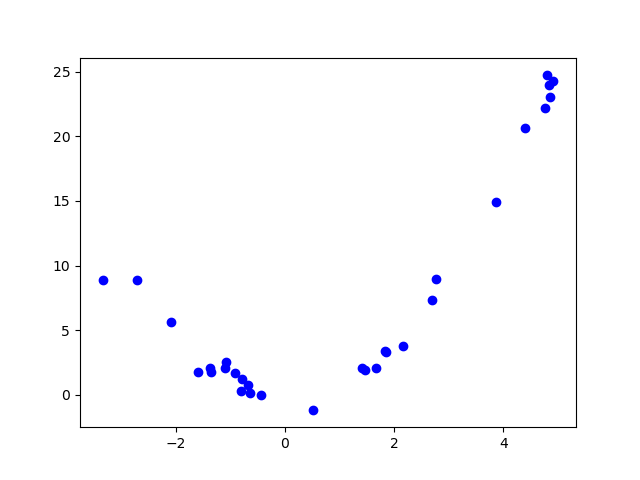
\includegraphics[width=0.5\textwidth]{../Figures/identifyModelGraph12A.png}
\end{center}
\begin{enumerate}[label=\Alph*.]
\item \( \text{Exponential model} \)
\item \( \text{Linear model} \)
\item \( \text{Non-linear Power model} \)
\item \( \text{Logarithmic model} \)
\item \( \text{None of the above} \)

\end{enumerate} }
\litem{
For the scenario below, use the model for the volume of a cylinder as $V = \pi r^2 h$ to find the coefficient for the model of the new volume $V_{\text{new}} = k r^2 h$.
\begin{center}
    \textit{ Pepsi wants to increase the volume of soda in their cans. They've decided to increase the radius by 12 percent and increase the height by 15 percent. They want to model the new volume based on the radius and height of the original cans. }
\end{center}
\begin{enumerate}[label=\Alph*.]
\item \( k = 0.00216 \)
\item \( k = 4.53194 \)
\item \( k = 1.44256 \)
\item \( k = 0.00679 \)
\item \( \text{None of the above.} \)

\end{enumerate} }
\litem{
For the scenario below, use the model for the volume of a cylinder as $V = \pi r^2 h$.
\begin{center}
    \textit{ Pringles wants to add 48 \text{percent} more chips to their cylinder cans and minimize the design change of their cans. They've decided that the best way to minimize the design change is to increase the radius and height by the same percentage. What should this increase be? }
\end{center}
\begin{enumerate}[label=\Alph*.]
\item \( \text{About } 22 \text{ percent} \)
\item \( \text{About } 4 \text{ percent} \)
\item \( \text{About } 24 \text{ percent} \)
\item \( \text{About } 14 \text{ percent} \)
\item \( \text{None of the above} \)

\end{enumerate} }
\litem{
Solve the modeling problem below, if possible.
\begin{center}
    \textit{ In CHM2045L, Brittany created a 19 liter 35 percent solution of chemical $\chi$ using two different solution percentages of chemical $\chi$. When she went to write her lab report, she realized she forgot to write the amount of each solution she used! If she remembers she used 20 percent and 42 percent solutions, what was the amount she used of the 20 percent solution? }
\end{center}
\begin{enumerate}[label=\Alph*.]
\item \( 11.11 liters \)
\item \( 9.50 liters \)
\item \( 12.95 liters \)
\item \( 6.05 liters \)
\item \( \text{There is not enough information to solve the problem.} \)

\end{enumerate} }
\litem{
Determine the appropriate model for the graph of points below.
\begin{center}
    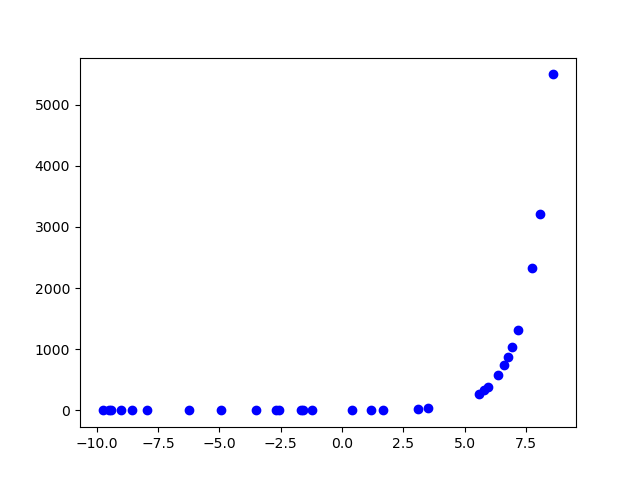
\includegraphics[width=0.5\textwidth]{../Figures/identifyModelGraph12CopyA.png}
\end{center}
\begin{enumerate}[label=\Alph*.]
\item \( \text{Non-linear Power model} \)
\item \( \text{Linear model} \)
\item \( \text{Logarithmic model} \)
\item \( \text{Exponential model} \)
\item \( \text{None of the above} \)

\end{enumerate} }
\litem{
Solve the modeling problem below, if possible.
\begin{center}
    \textit{ A new virus is spreading throughout the world. There were initially 8 many cases reported, but the number of confirmed cases has quadrupled every 3 days. How long will it be until there are at least 1000000 confirmed cases? }
\end{center}
\begin{enumerate}[label=\Alph*.]
\item \( \text{About } 12 \text{ days} \)
\item \( \text{About } 26 \text{ days} \)
\item \( \text{About } 36 \text{ days} \)
\item \( \text{About } 14 \text{ days} \)
\item \( \text{There is not enough information to solve the problem.} \)

\end{enumerate} }
\litem{
Solve the modeling problem below, if possible.
\begin{center}
    \textit{ A new virus is spreading throughout the world. There were initially 7 many cases reported, but the number of confirmed cases has quadrupled every 4 days. How long will it be until there are at least 1000 confirmed cases? }
\end{center}
\begin{enumerate}[label=\Alph*.]
\item \( \text{About } 15 \text{ days} \)
\item \( \text{About } 20 \text{ days} \)
\item \( \text{About } 10 \text{ days} \)
\item \( \text{About } 9 \text{ days} \)
\item \( \text{There is not enough information to solve the problem.} \)

\end{enumerate} }
\litem{
For the scenario below, use the model for the volume of a cylinder as $V = \pi r^2 h$.
\begin{center}
    \textit{ Pringles wants to add 41 \text{percent} more chips to their cylinder cans and minimize the design change of their cans. They've decided that the best way to minimize the design change is to increase the radius and height by the same percentage. What should this increase be? }
\end{center}
\begin{enumerate}[label=\Alph*.]
\item \( \text{About } 20 \text{ percent} \)
\item \( \text{About } 19 \text{ percent} \)
\item \( \text{About } 3 \text{ percent} \)
\item \( \text{About } 12 \text{ percent} \)
\item \( \text{None of the above} \)

\end{enumerate} }
\litem{
Using the scenario below, model the population of bacteria $\alpha$ in terms of the number of minutes, $t$ that pass. Then, choose the correct approximate \textit{(rounded to the nearest minute)} replication rate of bacteria-$\alpha$.
\begin{center}
    \textit{ A newly discovered bacteria, $\alpha$, is being examined in a lab. The lab started with a petri dish of 4 bacteria-$\alpha$. After 3 hours, the petri dish has 19753 bacteria-$\alpha$. Based on similar bacteria, the lab believes bacteria-$\alpha$ triples after some undetermined number of minutes. }
\end{center}
\begin{enumerate}[label=\Alph*.]
\item \( \text{About } 14 \text{ minutes} \)
\item \( \text{About } 227 \text{ minutes} \)
\item \( \text{About } 88 \text{ minutes} \)
\item \( \text{About } 37 \text{ minutes} \)
\item \( \text{None of the above} \)

\end{enumerate} }
\litem{
Solve the modeling problem below, if possible.
\begin{center}
    \textit{ In CHM2045L, Brittany created a 28 liter 34 percent solution of chemical $\chi$ using two different solution percentages of chemical $\chi$. When she went to write her lab report, she realized she forgot to write the amount of each solution she used! If she remembers she used 20 percent and 36 percent solutions, what was the amount she used of the 36 percent solution? }
\end{center}
\begin{enumerate}[label=\Alph*.]
\item \( 24.50 liters \)
\item \( 3.26 liters \)
\item \( 3.50 liters \)
\item \( 14.00 liters \)
\item \( \text{There is not enough information to solve the problem.} \)

\end{enumerate} }
\litem{
Determine the appropriate model for the graph of points below.
\begin{center}
    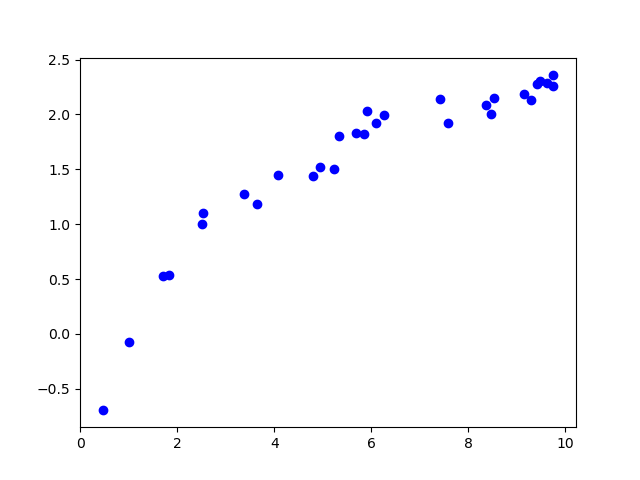
\includegraphics[width=0.5\textwidth]{../Figures/identifyModelGraph12B.png}
\end{center}
\begin{enumerate}[label=\Alph*.]
\item \( \text{Linear model} \)
\item \( \text{Logarithmic model} \)
\item \( \text{Exponential model} \)
\item \( \text{Non-linear Power model} \)
\item \( \text{None of the above} \)

\end{enumerate} }
\litem{
For the information provided below, construct a linear model that describes the total distance of the path, $D$, in terms of the time spent on a particular path \textit{if we know that the time spent on each path was equal}.
\begin{center}
    \textit{ A bicyclist is training for a race on a hilly path. Their bike keeps track of their speed at any time, but not the distance traveled. Their speed traveling up a hill is 6 mph, 10 mph when traveling down a hill, and 8 mph when traveling along a flat portion. }
\end{center}
\begin{enumerate}[label=\Alph*.]
\item \( 0.392 t \)
\item \( 480 t \)
\item \( 24 t \)
\item \( \text{The model can be found with the information provided, but isn't options 1-3.} \)
\item \( \text{The model cannot be found with the information provided.} \)

\end{enumerate} }
\litem{
For the scenario below, use the model for the volume of a cylinder as $V = \pi r^2 h$.
\begin{center}
    \textit{ Pringles wants to add 30 \text{percent} more chips to their cylinder cans and minimize the design change of their cans. They've decided that the best way to minimize the design change is to increase the radius and height by the same percentage. What should this increase be? }
\end{center}
\begin{enumerate}[label=\Alph*.]
\item \( \text{About } 15 \text{ percent} \)
\item \( \text{About } 14 \text{ percent} \)
\item \( \text{About } 9 \text{ percent} \)
\item \( \text{About } 3 \text{ percent} \)
\item \( \text{None of the above} \)

\end{enumerate} }
\litem{
Solve the modeling problem below, if possible.
\begin{center}
    \textit{ In CHM2045L, Brittany created a 27 liter 27 percent solution of chemical $\chi$ using two different solution percentages of chemical $\chi$. When she went to write her lab report, she realized she forgot to write the amount of each solution she used! If she remembers she used 16 percent and 37 percent solutions, what was the amount she used of the 16 percent solution? }
\end{center}
\begin{enumerate}[label=\Alph*.]
\item \( 13.39 liters \)
\item \( 12.86 liters \)
\item \( 13.50 liters \)
\item \( 14.14 liters \)
\item \( \text{There is not enough information to solve the problem.} \)

\end{enumerate} }
\litem{
Determine the appropriate model for the graph of points below.
\begin{center}
    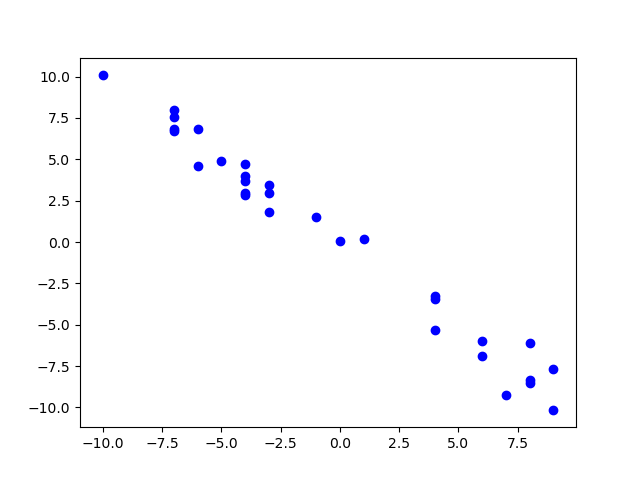
\includegraphics[width=0.5\textwidth]{../Figures/identifyModelGraph12CopyB.png}
\end{center}
\begin{enumerate}[label=\Alph*.]
\item \( \text{Non-linear Power model} \)
\item \( \text{Linear model} \)
\item \( \text{Exponential model} \)
\item \( \text{Logarithmic model} \)
\item \( \text{None of the above} \)

\end{enumerate} }
\litem{
Solve the modeling problem below, if possible.
\begin{center}
    \textit{ A new virus is spreading throughout the world. There were initially 8 many cases reported, but the number of confirmed cases has doubled every 3 days. How long will it be until there are at least 1000000 confirmed cases? }
\end{center}
\begin{enumerate}[label=\Alph*.]
\item \( \text{About } 14 \text{ days} \)
\item \( \text{About } 51 \text{ days} \)
\item \( \text{About } 36 \text{ days} \)
\item \( \text{About } 15 \text{ days} \)
\item \( \text{There is not enough information to solve the problem.} \)

\end{enumerate} }
\litem{
Solve the modeling problem below, if possible.
\begin{center}
    \textit{ A new virus is spreading throughout the world. There were initially 8 many cases reported, but the number of confirmed cases has doubled every 3 days. How long will it be until there are at least 1000000 confirmed cases? }
\end{center}
\begin{enumerate}[label=\Alph*.]
\item \( \text{About } 36 \text{ days} \)
\item \( \text{About } 51 \text{ days} \)
\item \( \text{About } 15 \text{ days} \)
\item \( \text{About } 14 \text{ days} \)
\item \( \text{There is not enough information to solve the problem.} \)

\end{enumerate} }
\litem{
For the scenario below, use the model for the volume of a cylinder as $V = \pi r^2 h$.
\begin{center}
    \textit{ Pringles wants to add 34 \text{percent} more chips to their cylinder cans and minimize the design change of their cans. They've decided that the best way to minimize the design change is to increase the radius and height by the same percentage. What should this increase be? }
\end{center}
\begin{enumerate}[label=\Alph*.]
\item \( \text{About } 10 \text{ percent} \)
\item \( \text{About } 3 \text{ percent} \)
\item \( \text{About } 16 \text{ percent} \)
\item \( \text{About } 17 \text{ percent} \)
\item \( \text{None of the above} \)

\end{enumerate} }
\litem{
For the information provided below, construct a linear model that describes her total costs, $C$, as a function of the number of months, $x$ she is at UF. 
\begin{center}
    \textit{ Aubrey is a college student going into her first year at UF. She will receive Bright Futures, which covers her tuition plus a \$400 educational expense each year. Before college, Aubrey saved up \$11000. She knows she will need to pay \$700 in rent a month, \$70 for food a week, and \$40 in other weekly expenses. }
\end{center}
\begin{enumerate}[label=\Alph*.]
\item \( C(x) = 810 \)
\item \( C(x) = 810 x \)
\item \( C(x) = 1140 \)
\item \( C(x) = 1140 x \)
\item \( \text{None of the above.} \)

\end{enumerate} }
\litem{
Solve the modeling problem below, if possible.
\begin{center}
    \textit{ In CHM2045L, Brittany created a 28 liter 34 percent solution of chemical $\chi$ using two different solution percentages of chemical $\chi$. When she went to write her lab report, she realized she forgot to write the amount of each solution she used! If she remembers she used 14 percent and 41 percent solutions, what was the amount she used of the 14 percent solution? }
\end{center}
\begin{enumerate}[label=\Alph*.]
\item \( 12.40 liters \)
\item \( 7.26 liters \)
\item \( 20.74 liters \)
\item \( 14.00 liters \)
\item \( \text{There is not enough information to solve the problem.} \)

\end{enumerate} }
\litem{
Determine the appropriate model for the graph of points below.
\begin{center}
    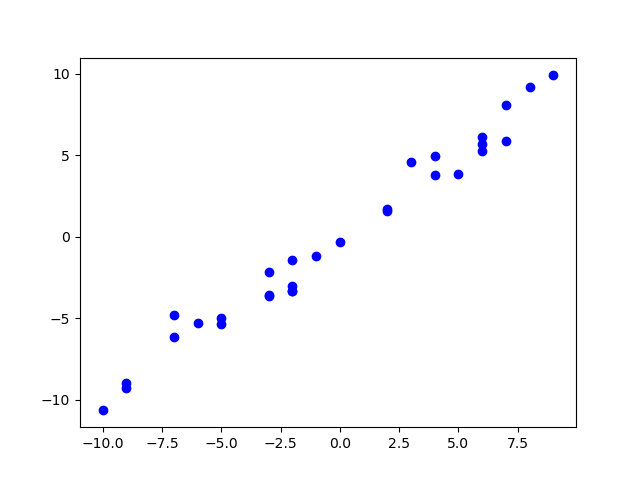
\includegraphics[width=0.5\textwidth]{../Figures/identifyModelGraph12C.png}
\end{center}
\begin{enumerate}[label=\Alph*.]
\item \( \text{Linear model} \)
\item \( \text{Logarithmic model} \)
\item \( \text{Non-linear Power model} \)
\item \( \text{Exponential model} \)
\item \( \text{None of the above} \)

\end{enumerate} }
\litem{
For the scenario below, model the rate of vibration (cm/s) of the string in terms of the length of the string. Then determine the variation constant $k$ of the model (if possible). The constant should be in terms of cm and s.
\begin{center}
    \textit{ The rate of vibration of a string under constant tension varies based on the type of string and the length of the string. The rate of vibration of string $\omega$ increases as the square length of the string decreases. For example, when string $\omega$ is 3 mm long, the rate of vibration is 25 cm/s. }
\end{center}
\begin{enumerate}[label=\Alph*.]
\item \( k = 2.78 \)
\item \( k = 2.25 \)
\item \( k = 277.78 \)
\item \( k = 225.00 \)
\item \( \text{None of the above.} \)

\end{enumerate} }
\litem{
For the scenario below, use the model for the volume of a cylinder as $V = \pi r^2 h$.
\begin{center}
    \textit{ Pringles wants to add 35 \text{percent} more chips to their cylinder cans and minimize the design change of their cans. They've decided that the best way to minimize the design change is to increase the radius and height by the same percentage. What should this increase be? }
\end{center}
\begin{enumerate}[label=\Alph*.]
\item \( \text{About } 3 \text{ percent} \)
\item \( \text{About } 18 \text{ percent} \)
\item \( \text{About } 16 \text{ percent} \)
\item \( \text{About } 11 \text{ percent} \)
\item \( \text{None of the above} \)

\end{enumerate} }
\litem{
Solve the modeling problem below, if possible.
\begin{center}
    \textit{ In CHM2045L, Brittany created a 22 liter 13 percent solution of chemical $\chi$ using two different solution percentages of chemical $\chi$. When she went to write her lab report, she realized she forgot to write the amount of each solution she used! If she remembers she used 13 percent and 37 percent solutions, what was the amount she used of the 13 percent solution? }
\end{center}
\begin{enumerate}[label=\Alph*.]
\item \( 11.00 liters \)
\item \( 2.56 liters \)
\item \( 0.00 liters \)
\item \( 22.00 liters \)
\item \( \text{There is not enough information to solve the problem.} \)

\end{enumerate} }
\litem{
Determine the appropriate model for the graph of points below.
\begin{center}
    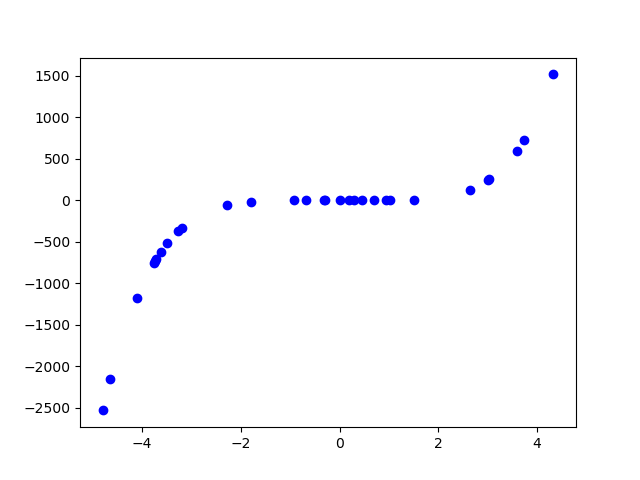
\includegraphics[width=0.5\textwidth]{../Figures/identifyModelGraph12CopyC.png}
\end{center}
\begin{enumerate}[label=\Alph*.]
\item \( \text{Linear model} \)
\item \( \text{Non-linear Power model} \)
\item \( \text{Exponential model} \)
\item \( \text{Logarithmic model} \)
\item \( \text{None of the above} \)

\end{enumerate} }
\end{enumerate}

\end{document}